\documentclass{beamer}
\usepackage[utf8]{inputenc}
\usepackage{hyperref}

\usepackage{tikz}

\usepackage{latexsym,xcolor,multicol,booktabs,calligra}
\usepackage{amsmath,amssymb,BOONDOX-cal,bm}	
\usepackage{graphicx,pstricks,stackengine} 
\usepackage{libertinus}
\usepackage{amssymb}
\usepackage{pgfplots}
\usepackage{tikz}
\usepackage{xcolor}
\usetikzlibrary{positioning}

\usepackage{hyperref}
\hypersetup{
    colorlinks=true,
    linkcolor=blue,
    urlcolor=blue,
    citecolor=blue
}

\usepackage{etoolbox}
\makeatletter
\newcommand{\noframenumbering}{%
  \beamer@noframenumberingtrue%
}
\makeatother

\usepackage[T1]{fontenc}

\title{Macroeconometrics\\
2 - AR(I)MA}
\author{Camille Souffron\\
Ecole Normale Supérieure \& Paris School of Economics\\
\textcolor{blue}{\href{mailto:camille.souffron@ens.psl.eu}{camille.souffron@ens.psl.eu}}}
\institute{\normalsize M2 EPOG JM}
\date{Fall 2026}

\usetheme{Singapore}

\def\cmd#1{\texttt{\color{red}\footnotesize $\backslash$#1}}
\def\env#1{\texttt{\color{RoyalBlue}\footnotesize #1}}

\newtheorem{thm}{Theorem}[theorem]
\setbeamertemplate{footline}[frame number]

\begin{document}

\begin{frame} % <-- no [plain] here!
    \titlepage % This keeps the theme style
    \begin{center}
        
\includegraphics[width=0.5\textwidth]{logos.png}
    \end{center}
\end{frame}



\addtocounter{framenumber}{-1}







\section{Introduction}



\begin{frame}{What We Have Learned So Far}
\scriptsize
\pause
\textbf{1. What is a Time Series?}
\begin{itemize}
    \item Ordered data over time: $(x_t)_{t=1}^T$
    \item Realization of an underlying stochastic process $(X_t)$
\end{itemize}
\pause
\textbf{2. Key Property: Time Dependence}
\begin{itemize}
    \item Time series are not i.i.d. $\Rightarrow$ dependence between $X_t$ and $X_{t-h}$ (and DGP distribution may change over time)
    \item Autocovariance $\gamma(h)$, Autocorrelation $\rho(h)$
    \item ACF as main empirical tool to detect persistence
\end{itemize}
\pause
\textbf{3. Stationarity: Why It Matters}
\begin{itemize}
    \item Weak stationarity: constant mean, variance, $\gamma(h)$ only depends on $h$, not on $t$
    \item Needed for LLN/CLT, inference, forecasting, and model estimation
    \item Ergodicity: time averages $\Rightarrow$ population moments
\end{itemize}
\pause
\textbf{4. Types of Nonstationarity}
\begin{itemize}
    \item Deterministic trend (trend‐stationary)
    \item Stochastic trend / unit root (difference‐stationary) - Unit root tests
    \item Seasonality, structural breaks
\end{itemize}
\pause
\textbf{5. Making Data Stationary}
\begin{itemize}
    \item Logs (variance stabilization), detrending (OLS) at different orders for trend-stat, differencing for diff-stat (= growth rate if in log), deseasonalizing
    \item Filters (HP, BK, CF): separate trend vs cycle but non‐neutral choice!
\end{itemize}
\pause
\textbf{6. Wold Theorem \& Motivation}
\begin{itemize}
    \item Any weakly stationary process admits linear MA($\infty$) representation
    \item Justifies AR/MA/ARMA models
\end{itemize}

\end{frame}


% ============================================================
%  MACROECONOMETRICS — AR, MA, and ARMA processes
%  (based on Doz & Ben Salem, M1 APE – Econometrics 2)
% ============================================================



\begin{frame}{}
  \centering
    \textbf{Now that we have stationary, detrended series, we can \textit{MODEL} the dynamics statistically.}
    
\vspace{0.3cm}

\textbf{To forecast, to simulate the impact of a shock (impulse response) etc...}

\end{frame}


\begin{frame}{}
  \centering
This week: univariate.

\vspace{0.3cm}

Next week: VAR.

\vspace{0.3cm}

\textbf{For next week, please read \textit{“A VAR Analysis for the Growth Regime and Demand Formation Patterns of the Japanese Economy”} (Hiroshi Nishi, 2021, \textit{Revue de la Régulation}) - available at \href{https://journals.openedition.org/regulation/9370}{https://journals.openedition.org/regulation/9370} - and send me \textbf{two questions by email} by \textbf{Tuesday noon}.}


\end{frame}





\begin{frame}{From Stationarity to Dynamic Models}
\begin{itemize}
    \item The vast majority of (weakly) stationary stochastic processes can often be represented as linear functions of past shocks.
    \item The Wold decomposition implies that any stationary process can be written as a deterministic part and an infinite moving average:
    \[
        X_t = \mu + \sum_{j=0}^{\infty} \psi_j \varepsilon_{t-j}, \quad \varepsilon_t \sim WN(0,\sigma^2)
    \]
    \item Truncating or inverting this representation yields finite-order linear models:
    \begin{align*}
        \text{AR}(p): &\quad X_t = \mu + \phi_1 X_{t-1} + \cdots + \phi_p X_{t-p} + \varepsilon_t\\
        \text{MA}(q): &\quad X_t = \mu + \varepsilon_t - \theta_1 \varepsilon_{t-1} - \cdots - \theta_q \varepsilon_{t-q}\\
        \text{ARMA}(p,q): &\quad \phi(L) X_t = \mu + \theta(L)\varepsilon_t
    \end{align*}
\end{itemize}
\end{frame}

\begin{frame}{Why Represent Time Series by AR and MA Models?}
\small
\textbf{Historical context: Box-Jenkins approach (1970) following Wold theorem (1938)}
\begin{itemize}
  \item \textbf{Goal:} find a \emph{finite}, parsimonious approximation of this infinite structure (without assuming \textit{structural relationships}!)
\end{itemize}

\pause
\textbf{Two natural truncations:}
\begin{itemize}
  \item Use past \textbf{values of $X$} $\rightarrow$ \textbf{Autoregressive (AR)} model.
  \item Use past \textbf{shocks $\varepsilon$} $\rightarrow$ \textbf{Moving Average (MA)} model.
  \item Combine both $\rightarrow$ \textbf{ARMA} model.
\end{itemize}

\pause
\textbf{Motivation:}
\begin{itemize}
  \item Capture short- and medium-term persistence with few parameters.
  \item Produce statistically efficient forecasts.
  \item Provide interpretable dynamic multipliers for shocks.
\end{itemize}

\end{frame}


\begin{frame}{The Best Linear Forecast (BLF)}

\textbf{Properties:}
\begin{itemize}
  \item The Wold theorem guarantees existence of the BLF for all stationary processes.
  \item Minimizes mean-square forecast error among all \emph{linear} predictors.
  \item The forecast error is orthogonal to all past values:
\[
\underbrace{\operatorname{Cov}(e_{t+h|t},\, X_{t-j})}_{\text{with forecast error } 
e_{t+h|t}=X_{t+h}-\hat{X}_t(h)} = 0, \quad \forall j \ge 0
\]
        \item AR, MA, ARMA models are finite-order approximations of this BLF.
\end{itemize}

\pause
\textbf{Connection with Wold Decomposition:}
\[
X_t = \sum_{j=0}^{\infty}\psi_j\varepsilon_{t-j}
\Rightarrow
\hat X_t(h) = \sum_{j=h}^{\infty}\psi_j\varepsilon_{t+h-j}.
\]
Thus, the Wold representation \emph{provides} the coefficients of the BLF.

\end{frame}

% ------------------------------------------------------------

\section{Lag Polynomials}
% ============================================================

\begin{frame}{The Lag Operator - Definition and Intuition}
\begin{itemize}
    \item The lag operator $L$ shifts a time series one period into the past:
    \[
        L X_t = X_{t-1}, \qquad L^k X_t = X_{t-k}.
    \]
    \item Using $L$ allows us to express temporal dependence algebraically:
    \[
        (1 - L)X_t = X_t - X_{t-1} \quad \text{(first difference operator)}.
    \]
    \item This makes dynamic relations concise and easier to manipulate, e.g.:
    \[
        (1 - \phi L) X_t = \varepsilon_t \quad \text{for an AR(1) process}.
    \]
\end{itemize}
\textbf{Intuition:} $L$ acts like a “time-shift operator.”  
Instead of writing $X_t = \phi X_{t-1} + \varepsilon_t$, we manipulate entire lag structures symbolically - just as we would with polynomials in algebra.
\end{frame}

% ------------------------------------------------------------

\begin{frame}{Lag Polynomials - Formal Definition}
\begin{itemize}
    \item A lag polynomial of order $p$ with real coefficients $\{\psi_i\}$ is:
    \[
        P(L) = \sum_{i=0}^{p} \psi_i L^i.
    \]
    When applied to a process $(X_t)$:
    \[
        P(L) X_t = \sum_{i=0}^{p} \psi_i X_{t-i}.
    \]
    \item For example, a moving-average process of order $q$ can be written as:
    \[
        X_t = \mu + \theta(L)\varepsilon_t, 
        \qquad \text{where } \theta(L) = 1 - \theta_1 L - \cdots - \theta_q L^q.
    \]
    \item Similarly, an autoregressive process ($p$) can be written as:
    \[
        \phi(L) X_t = \mu + \varepsilon_t, 
        \qquad \phi(L) = 1 - \phi_1 L - \cdots - \phi_p L^p.
    \]
\end{itemize}
\end{frame}

% ------------------------------------------------------------
\begin{frame}{Stability, Invertibility, and Roots of Lag Polynomials}
\small
\begin{itemize}
    \item The roots of a lag polynomial determine whether the process is stable (stationary) or explosive.
    \[
        \text{If } \phi(L) = 1 - \phi_1 L - \cdots - \phi_p L^p, 
        \quad \text{define } \phi(z) = 1 - \phi_1 z - \cdots - \phi_p z^p.
    \]
    \item The process is \textbf{stationary} if all roots $z_i$ satisfy $|z_i| > 1$.  
    (Equivalently, the associated $\lambda_i = 1/z_i$ satisfy $|\lambda_i| < 1$.)
    \item If any $|z_i| = 1$, the process has a \textbf{unit root} (random walk, stochastic trend).  
      If some $|z_i| < 1$, it is \textbf{explosive}.
    \item For \textbf{invertibility} (MA side), we require the same condition on the $\theta(z)$ polynomial.
\end{itemize}
\end{frame}

% ------------------------------------------------------------
\begin{frame}{Stability, Invertibility, and Roots of Lag Polynomials}
\small
\textbf{Inversion of the polynomial.}
\[
\text{If all } |\lambda_i| < 1, \quad \phi(L)^{-1} = 
(1 - \phi_1 L - \cdots - \phi_p L^p)^{-1} 
= \sum_{k=0}^{\infty} a_k L^k,
\]
where the coefficients $a_k$ follow the recursion
\[
a_k = \phi_1 a_{k-1} + \phi_2 a_{k-2} + \cdots + \phi_p a_{k-p}, \quad a_0 = 1.
\]
Thus, any AR($p$) process admits an \textbf{MA($\infty$) representation}:
\[
X_t = \sum_{k=0}^{\infty} a_k \varepsilon_{t-k}, \qquad 
\sum_k |a_k| < \infty \text{ if all } |\lambda_i|<1.
\]

\textbf{Intuition:}  
The AR polynomial governs how past values feed into the present.  
If all feedback roots lie outside the unit circle, the inverse polynomial converges,  
past effects die out, and the system “forgets” its history.
\end{frame}


\begin{frame}{Stability, Invertibility, and Roots of Lag Polynomials}

\textbf{Example:} For an AR(1) process, it is direct (through $\lambda$). \( X_t = \lambda X_{t-1} + \varepsilon_t \)
\[
(1 - \lambda L) X_t = \varepsilon_t.
\]
\begin{itemize}
    \item If $|\lambda| < 1$: the effect of shocks dies out exponentially.  
      The process is stationary and mean-reverting.
    \item If $|\lambda| = 1$: shocks accumulate $\to$ a random walk (non-stationary).
    \item If $|\lambda| > 1$: shocks amplify $\to$ explosive dynamics.
\end{itemize}

\textbf{Intuition:}  
The lag polynomial encodes how today’s $X_t$ depends on its past.  
If the “feedback” coefficients sum to less than one in magnitude, past influences fade away; otherwise, they persist or blow up.

\end{frame}


% ------------------------------------------------------------
\section{AR(p)}

% ============================================================
\begin{frame}{The AR(1) Case}
\small


\textbf{Inversion (limit of a geometric series) and MA($\infty$) Representation}\footnote{
Why: same logic as the geometric series 
$\frac{1}{1-\lambda} = \sum_{k=0}^{\infty}\lambda^k$ for $|\lambda|<1$.
Indeed,
$(1-\lambda)\big(1+\lambda+\lambda^2+\cdots\big)
=1+ \lambda + \lambda^2 + \cdots 
- (\lambda + \lambda^2 + \lambda^3 + \cdots) = 1$.
So the infinite sum is the inverse of $(1-\lambda)$.
Applying this to the lag operator gives 
$(1-\lambda L)^{-1}=1+\lambda L+\lambda^2 L^2+\cdots$.}

\[
(1 - \lambda L)^{-1} = 1 + \lambda L + \lambda^2 L^2 + \lambda^3 L^3 + \cdots
\]
\[
\Rightarrow \quad X_t = \varepsilon_t + \lambda \varepsilon_{t-1} + \lambda^2 \varepsilon_{t-2} + \cdots 
        = \sum_{k=0}^{\infty} \lambda^k \varepsilon_{t-k}.
\]
\begin{itemize}
    \item Converges only if $|\lambda|<1$.
    \item Each shock affects future values with weight $\lambda^k$.
    \item For $\lambda=0.8$, shocks decay geometrically at rate $0.8^k$.
\end{itemize}

\textbf{Interpretation:}  
The AR(1) process can be seen as an infinite moving average of past shocks,  
whose influence vanishes exponentially.

\end{frame}

% ------------------------------------------------------------

\begin{frame}{Geometric Intuition and Simple Numerical Example}
\begin{itemize}
    \item Suppose $\lambda = 0.8$.  
          Then $X_t =  \sum_{i=0}^{k-1} 0.8^i \varepsilon_{t-i}$.  
          As $k \to \infty$, $0.8^k \to 0$ and the effect of initial conditions disappears.
    \item If $\lambda = 1$, the term $X_{t-1}$ accumulates without bound:  
          $X_t = X_0 + \sum_{i=0}^{t-1}\varepsilon_i$ → variance variance $\mathrm{Var}(X_t)= \mathrm{Var}(\sum_{j=1}^t \varepsilon_j)=t\sigma^2$ grows linearly with $t$.
    \item If $\lambda = 1.1$, $X_t$ explodes exponentially because $1.1^t$ diverges.
\end{itemize}

\end{frame}


\begin{frame}{Why Inversion Works: Geometric-Series Intuition}
\small

\textbf{Reminder - Geometric Series:}
\[
\sum_{k=0}^{n-1} r^k = \frac{1 - r^n}{1 - r}
\quad \Rightarrow \quad
\sum_{k=0}^{\infty} r^k = \frac{1}{1 - r} \quad \text{if } |r| < 1.
\]

\medskip
\textbf{Intuition:} same logic applies to any AR($p$):
\[
\phi(L)^{-1} = \sum_{k=0}^{\infty} a_k L^k, \quad 
a_k = \phi_1 a_{k-1} + \cdots + \phi_p a_{k-p}.
\]
Convergence (and stability) holds only if all roots satisfy $|\lambda_i| < 1$,
so the “feedback” coefficients decay geometrically - past shocks die out.

\bigskip
\centering
\textit{$\to$ Stationarity = geometric damping of past influences.}
\end{frame}

\begin{frame}{Example Pipeline: AR(2) Process}
\smallskip
\textbf{Model:}
\[
X_t=\phi_1 X_{t-1}+\phi_2 X_{t-2}+\varepsilon_t,\qquad \varepsilon_t\sim WN(0,\sigma^2).
\]

\textbf{Lag polynomial:}\quad \(\phi(L)=1-\phi_1 L-\phi_2 L^2\).

\textbf{Step 1: Characteristic roots (lag domain).}
Solve
\[
\lambda^2-\phi_1\lambda-\phi_2=0 \quad\Rightarrow\quad \lambda_1,\lambda_2.
\]
\[
\text{Stationarity} \ \Longleftrightarrow\ |\lambda_1|<1\ \text{and}\ |\lambda_2|<1.
\]

\textbf{Step 2: Inversion and MA($\infty$).}
If $|\lambda_i|<1$,
\[
(1-\phi_1 L-\phi_2 L^2)^{-1}=\sum_{k=0}^{\infty} a_k L^k,\qquad
a_k=\frac{\lambda_1^{k+1}-\lambda_2^{k+1}}{\lambda_1-\lambda_2}.
\]
Hence
\[
X_t=\sum_{k=0}^{\infty} a_k\,\varepsilon_{t-k}.
\]
\end{frame}


\begin{frame}{Example Pipeline: AR(2) Process}
\smallskip
\textbf{Step 3: Numerical examples}

\textbf{Case 1:} $\phi_1=1.3,\ \phi_2=-0.4$.
\[
\lambda^2-1.3\lambda+0.4=0 \ \Rightarrow\ \lambda_{1,2}=0.8,\ 0.5.
\]
Both $|\lambda_i|<1$ $\Rightarrow$ \textbf{stationary}.


\textbf{Case 2:} $\phi_1=0.7,\ \phi_2=-0.2$.
\[
\lambda^2-0.7\lambda+0.2=0 \ \Rightarrow\ \lambda_{1,2}=0.35\pm0.278i,
\]

\[ |\lambda_i|=\sqrt{0.35^2+0.278^2}\approx 0.447<1\]

$\Rightarrow$ \textbf{stationary (complex conjugate roots inside unit circle)} Interpret?
\pause
\vspace{0.3em}
\textbf{\textit{Complex roots imply damped oscillations in the impulse response.}}
\end{frame}


% ------------------------------------------------------------

\subsection{Autoregressive Processes AR(p)}

\begin{frame}{AR(p): Definition and Canonical Form}
\[
    X_t = \mu + \phi_1 X_{t-1} + \cdots + \phi_p X_{t-p} + \varepsilon_t, 
    \quad \varepsilon_t \sim WN(0,\sigma^2)
\]
or equivalently \( \phi(L) X_t = \mu + \varepsilon_t \), with \( \phi(L) = 1 - \phi_1 L - \cdots - \phi_p L^p \).

\begin{itemize}
    \item Mean: \( \mathbb{E}[X_t] = \mu / (1 - \sum_{i=1}^p \phi_i) \)
    \item Stationarity condition: all roots of \( \phi(z) = 0 \) satisfy \( |z| > 1 \)
    \item Under stationarity, AR(p) has an infinite MA representation:
    \[
        X_t = m + \sum_{k=0}^{\infty} a_k \varepsilon_{t-k}, 
        \quad \sum_k |a_k| < \infty
    \]
\end{itemize}

\end{frame}

% ------------------------------------------------------------

\section{MA(q)}

\begin{frame}{Moving Average (MA) Process}
\footnotesize
\textbf{Definition (MA($q$)):}
\[
X_t = \mu + \varepsilon_t - \theta_1 \varepsilon_{t-1} - \cdots - \theta_q \varepsilon_{t-q}, 
\quad \varepsilon_t \sim WN(0,\sigma^2).
\]
\footnote{\scriptsize \textbf{Sign convention (Box-Jenkins):} $\theta(L)=1-\theta_1 L-\cdots-\theta_q L^q$. Some software (e.g.\ Stata, some R packages) use $+\theta_j$ in the model, giving opposite signs in reported coefficients. Always check the documentation.}

\begin{itemize}
    \item Each $X_t$ is a finite weighted sum of current and past shocks.
    \item No feedback from past $X$’s → \textbf{always stationary} for any finite $q$.
    \item Stationarity holds even if some $\theta_i$ are large or negative, because 
    shocks enter with finite weights and finite variance.
\end{itemize}

\textbf{Roots and unit roots:}
\[
\theta(L) = 1 - \theta_1 L - \cdots - \theta_q L^q,
\quad \theta(z) = 0.
\]
\begin{itemize}
    \item A \textbf{unit root} ($|z_i|=1$) makes $\theta(L)$ non-invertible.
    \item If any $|z_i|<1$, the process is still stationary but \emph{not invertible}: the underlying shocks $\varepsilon_t$ cannot be recovered uniquely.
\end{itemize}
\end{frame}

% ------------------------------------------------------------
\begin{frame}{Moving Average (MA) Process}
\textbf{Summary:}
\begin{center}
\begin{tabular}{lcc}
\toprule
Property & Condition & Consequence \\
\midrule
Stationarity & Always (finite $q$) & Finite-variance process \\
Invertibility & $|z_i|>1$ & Unique MA representation \\
Unit root & $|z_i|=1$ & Non-invertible, non-identifiable \\
\bottomrule
\end{tabular}
\end{center}
\end{frame}

% ------------------------------------------------------------
\begin{frame}{Invertibility of the MA($q$) Process}
\small

\textbf{Motivation}  
All finite MA($q$) processes are \textbf{stationary}, since each $X_t$ is a finite
linear combination of white noise shocks.  
However, to identify the shocks $\varepsilon_t$ uniquely from the data,
we require an additional property called \textbf{invertibility}.

\bigskip
\textbf{Formal setup}
\[
X_t = \theta(L)\varepsilon_t, 
\qquad \theta(L) = 1 - \theta_1 L - \cdots - \theta_q L^q.
\]
The corresponding polynomial is $\theta(z)=1-\theta_1 z-\cdots-\theta_q z^q$.

\pause
\textbf{Invertibility condition}  
If all roots $z_i$ of $\theta(z)=0$ satisfy $|z_i|>1$,
then the inverse polynomial $\theta(L)^{-1}$ admits a
convergent power-series expansion:
\[
\theta(L)^{-1}=1+\psi_1 L+\psi_2 L^2+\psi_3 L^3+\cdots ,
\]
and we can recover the shocks as a stable infinite AR of the observed data:
\[
\varepsilon_t = X_t + \psi_1 X_{t-1} + \psi_2 X_{t-2} + \cdots 
               = \sum_{k=0}^{\infty} \psi_k X_{t-k}.
\]
\end{frame}

% ------------------------------------------------------------
\begin{frame}{Invertibility of the MA($q$) Process}
\footnotesize

Hence the MA($q$) admits an equivalent AR($\infty$) representation:
\[
X_t = \sum_{k=1}^{\infty} \phi_k X_{t-k} + \varepsilon_t.
\]
\pause
\textbf{If non-invertible:}
\begin{itemize}
    \item The series for $\theta(L)^{-1}$ diverges (\emph{not} $X_t$ itself).  
    \item $X_t$ remains stationary, but $\varepsilon_t$ is no longer uniquely defined - many shock sequences can generate the same data.
    \item Inference becomes ill-posed: likelihood functions are not unique.
\end{itemize}

\pause
\textbf{Example (MA(1)):}
\[
X_t = \varepsilon_t - \theta \varepsilon_{t-1}.
\]
\begin{itemize}
    \item If $|\theta|<1$, \; $(1-\theta L)^{-1}=1+\theta L+\theta^2 L^2+\cdots$ converges:
    \[
        \varepsilon_t = X_t + \theta X_{t-1} + \theta^2 X_{t-2} + \cdots.
    \]
    \item If $|\theta|>1$, the inverse diverges;  
          equivalently, we can rewrite the process as
          \( X_t = \tilde{\varepsilon}_t - \tilde{\theta}\tilde{\varepsilon}_{t-1} \)
          with \( \tilde{\theta}=1/\theta \) and \( \tilde{\varepsilon}_t=-\theta\varepsilon_t \),
          restoring invertibility.
\end{itemize}

\textbf{Summary:}  
Stationarity concerns the finiteness of $X_t$; invertibility concerns the uniqueness and convergence of the innovation representation.

\end{frame}




% ------------------------------------------------------------

\section{ARMA}
\begin{frame}{ARMA($p,q$) Process - Definition and Intuition}
\small

\textbf{General form:}
\[
\phi(L)(X_t - \mu) = \theta(L)\varepsilon_t,
\]
where 
\[
\phi(L) = 1 - \phi_1 L - \cdots - \phi_p L^p, 
\quad \theta(L) = 1 - \theta_1 L - \cdots - \theta_q L^q,
\quad \varepsilon_t \sim WN(0,\sigma^2).
\]

\pause
\textbf{Stationarity and Invertibility:}
\begin{itemize}
    \item \textbf{Stationary} $\iff$ all roots of $\phi(z)=0$ lie outside the unit circle  
          $\to$ past values of $X_t$ don’t cause divergence.
    \item \textbf{Invertible} $\iff$ all roots of $\theta(z)=0$ lie outside the unit circle  
          $\to$ the innovations $\varepsilon_t$ can be uniquely recovered from $X_t$.
\end{itemize}
\end{frame}

% ------------------------------------------------------------
\begin{frame}{ARMA($p,q$) Process - Definition and Intuition}
\small

\textbf{Infinite representations: ARMA(p,q) = MA($\infty$) and AR($\infty$)}
\[
\text{(MA($\infty$))} \quad X_t = \mu + \sum_{j=0}^{\infty} \psi_j \varepsilon_{t-j},
\qquad
\text{(AR($\infty$))} \quad \varepsilon_t = X_t - \sum_{j=1}^{\infty} \pi_j X_{t-j}.
\]

\textbf{Intuition:}
\begin{itemize}
    \item The \textbf{MA($\infty$)} form shows $X_t$ as the cumulative effect of all past shocks  
          $\to$ how the system \emph{propagates and fades} random disturbances over time.
    \item The \textbf{AR($\infty$)} form shows $\varepsilon_t$ as what remains after removing a long memory of past values  
          $\to$ how the system \emph{filters out predictable components}.
    \item Both representations are equivalent when stationarity and invertibility hold:  
          every ARMA is a “shock-filtering” system that smooths white noise into persistent dynamics.
\end{itemize}

\textit{Economically:} shocks $\varepsilon_t$ represent structural innovations (policy, demand, etc.),  
and $\psi_j$ coefficients describe their delayed impacts - i.e. the dynamic multiplier path.

\end{frame}

\begin{frame}{Moments, ACF, and PACF in Stationary Time Series}
\small
\textbf{1. Moments of a weakly stationary process:}
\[
\mathbb{E}[X_t] = \mu, \qquad
\mathrm{Var}(X_t) = \gamma(0), \qquad
\mathrm{Cov}(X_t, X_{t-h}) = \gamma(h),
\]
where $\gamma(h)$ depends only on the lag $h$, not on $t$.

\pause
\textbf{2. Autocorrelation Function (ACF):}
\[
\rho(h) = \frac{\gamma(h)}{\gamma(0)}, \quad
\rho(0)=1.
\]
\begin{itemize}
    \item Measures the \textbf{linear dependence} between $X_t$ and its past $X_{t-h}$.
    \item Interpreted as “memory” or persistence over lag $h$.
    \item Empirical estimate: $\widehat\rho(h) = \frac{\sum_t (X_t-\bar X)(X_{t-h}-\bar X)}{\sum_t (X_t-\bar X)^2}$.
\end{itemize}
\end{frame}


\begin{frame}{Moments, ACF, and PACF in Stationary Time Series}
\small
\textbf{3. Partial Autocorrelation Function (PACF):}
\[
\phi_{hh} = \text{Corr}\big(X_t, X_{t-h} \,\big|\, X_{t-1}, \ldots, X_{t-h+1}\big).
\]
\begin{itemize}
    \item Measures the \textbf{direct link} between $X_t$ and $X_{t-h}$, 
          controlling for intermediate lags.
    \item Equivalently, the coefficient of $X_{t-h}$ in the best linear regression
          of $X_t$ on $(X_{t-1},\dots,X_{t-h})$.
\end{itemize}

\pause
\textbf{Interpretation:}
\begin{itemize}
    \item ACF $\to$ overall persistence (total correlation, indirect + direct).
    \item PACF $\to$ \emph{net} correlation at lag $h$ (direct link only).
    \item Stationary processes: both decay to 0 as $h \to \infty$.
\end{itemize}

\end{frame}


\begin{frame}{Moments of AR(1) and ARMA Processes}
\small
\textbf{Example: AR(1) process}
\[
X_t = \mu + \phi X_{t-1} + \varepsilon_t, \qquad \varepsilon_t \sim WN(0,\sigma^2).
\]

\textbf{Moments:}
\[
\mathbb{E}[X_t] = \frac{\mu}{1-\phi}, \quad
\mathrm{Var}(X_t) = \frac{\sigma^2}{1-\phi^2}, \quad
\rho(h) = \phi^h.
\]

\pause
\textbf{Interpretation:}
\begin{itemize}
    \item $\phi$ controls the persistence of autocorrelation.
    \item As $|\phi| \to 1$, the process becomes highly persistent.
    \item The ACF decays exponentially - typical of mean-reverting dynamics.
\end{itemize}

\pause
\textbf{For ARMA($p,q$):}
\[
\gamma(h) = \sum_{i=1}^p \phi_i \gamma(h-i)
            + \sigma^2 \sum_{j=0}^{q-h} \theta_j \theta_{j+h}.
\]

\end{frame}





\section{Identification}


\begin{frame}{Identification via ACF and PACF}
\small
\textbf{Why ACF/PACF?}
\begin{itemize}
    \item Before estimation, we must identify appropriate $(p,q)$ orders.
    \item Sample \textbf{autocorrelation function (ACF)} and \textbf{partial autocorrelation function (PACF)} 
          help detect underlying AR or MA structures.
\end{itemize}
\medskip
\textbf{Typical patterns:}
\centering
\begin{tabular}{lccc}
\toprule
Model & Stationarity & ACF Pattern & PACF Pattern \\
\midrule
AR(p) & $|\phi_i|<1$ & Exponential decay& Cutoff at $p$ \\
MA(q) & Always & Cutoff at $q$ & Exponential decay\\
ARMA(p,q) & $|\phi_i|<1$ & Exponential decay& Exponential decay\\
\bottomrule
\end{tabular}
\medskip
Use the cutoff/decay patterns to guess $(p,q)$.
\end{frame}

\begin{frame}{Identification via ACF and PACF}
\centering
\begin{tabular}{lccc}
\toprule
Model & Stationarity & ACF Pattern & PACF Pattern \\
\midrule
AR($p$)  & $|\phi_i|<1$ & Exponential decay& Cutoff after lag $p$ \\
MA($q$)  & Always        & Cutoff after lag $q$ & Exponential decay\\
ARMA($p,q$) & $|\phi_i|<1$ & Exponential decay& Exponential decay\\
\bottomrule
\end{tabular}

\medskip
\smallskip
\raggedright
\begin{itemize}
    \item \textbf{AR($p$):} each $X_t$ depends recursively on its own past $\to$ correlations
    at all horizons, but increasingly weaker (geometric decay).  
    Once you control for the first $p$ lags, no additional direct link remains ⇒ PACF cuts off.
    \item \textbf{MA($q$):} $X_t$ depends on a finite number of past shocks $\varepsilon_{t-j}$,
    so correlations vanish beyond $q$ lags.  
 However, partial correlations remain because each new lag still removes indirect noise dependence $\to$ PACF decays gradually.
    \item \textbf{ARMA($p,q$):} mix of both - infinite but damped memory from the AR part,
    finite shock smoothing from the MA part $\to$ both ACF and PACF decay smoothly.
\end{itemize}
\end{frame}

\begin{frame}{Identification via ACF and PACF}
\begin{figure}
    \centering
    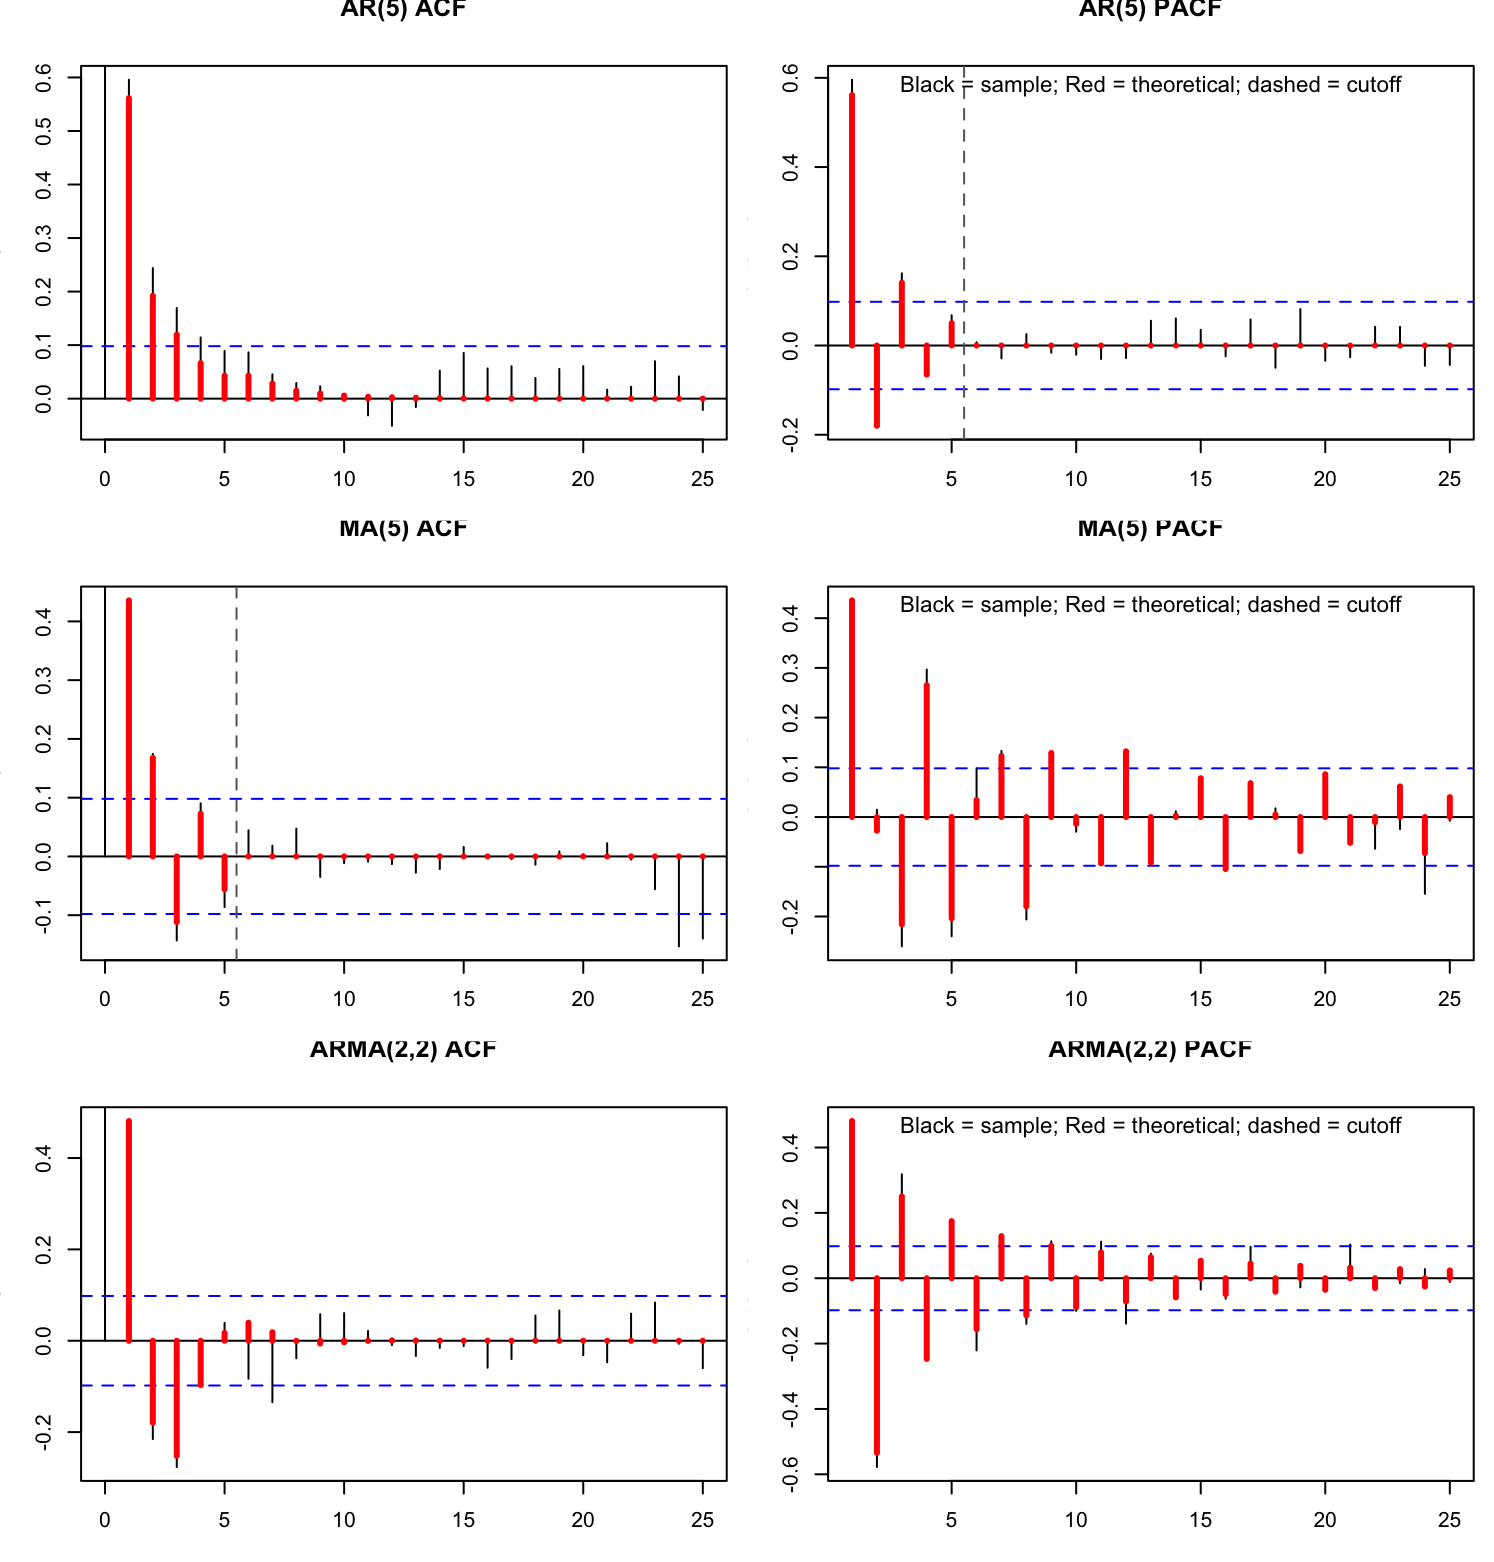
\includegraphics[width=0.7\linewidth]{ACF_PACF_id.png}
\end{figure}
    
\end{frame}


\section{Estimation}


\begin{frame}{Estimation of AR, MA and ARMA Models}
\small
\textbf{AR($p$):}
\[
X_t = \phi_1 X_{t-1} + \cdots + \phi_p X_{t-p} + \varepsilon_t.
\]
\begin{itemize}
  \item Regressors ($X_{t-1},\dots,X_{t-p}$) are observed and depend only on past shocks.
  \item \textbf{Are the regressors correlated with} $\varepsilon_t$?

\end{itemize}
\end{frame}


\begin{frame}{Estimation of AR, MA and ARMA Models}
\small
\textbf{AR($p$):}
\[
X_t = \phi_1 X_{t-1} + \cdots + \phi_p X_{t-p} + \varepsilon_t.
\]
\begin{itemize}
  \item Regressors ($X_{t-1},\dots,X_{t-p}$) are observed and depend only on past shocks. We assume $\varepsilon_t$ a white noise.
  \item $\Rightarrow$ Uncorrelated with $\varepsilon_t$ (since \textbf{NO EXPECTATION} (not a \textit{structural} model) → OLS is consistent.
  \item Same as a standard linear regression.
\end{itemize}

\pause
\textbf{MA($q$):}
\[
X_t = \varepsilon_t - \theta_1 \varepsilon_{t-1} - \cdots - \theta_q \varepsilon_{t-q}.
\]
\begin{itemize}
  \item Regressors ($\varepsilon_{t-1},\varepsilon_{t-2},\dots$) are \emph{unobserved}.
  \item $\Rightarrow$ Cannot apply OLS; endogeneity ($\mathbb{E}[\varepsilon_{t-1} X_t] \neq 0$)
 + latent variables ($\varepsilon_{t-1}$ not observable). 
  \item Need \textbf{Maximum Likelihood Estimation (MLE)} or \textbf{Nonlinear Least Squares (NLS)}:

\end{itemize}
\end{frame}


\begin{frame}{Estimation of AR, MA and ARMA Models}
\small

Need \textbf{Maximum Likelihood Estimation (MLE)} or \textbf{Nonlinear Least Squares (NLS)}:
  \[
  \hat{\theta} = \arg\min_\theta \sum_t \varepsilon_t(\theta)^2,
  \quad \varepsilon_t(\theta) = X_t + \sum_{i=1}^q \theta_i \varepsilon_{t-i}(\theta).
  \]
  
\textbf{ ARMA($p,q$): MLE, then.}
 
\textbf{Summary:}
\begin{center}
\begin{tabular}{lccc}
\toprule
Model & Observable regressors & OLS valid? & Estimation method \\
\midrule
AR($p$) & Yes & Yes& OLS / ML\\
MA($q$) & No & No& ML / NLS / Kalman filter \\
ARMA($p,q$) & No& No& ML / Kalman filter \\
\bottomrule
\end{tabular}
\end{center}
\end{frame}


% ------------------------------------------------------------
\begin{frame}{A brief note on Maximum Likelihood Estimation (MLE)}
\small

\textbf{Idea:}  
Choose the parameters that make the observed data \(\{X_t\}_{t=1}^T\) the \emph{most likely} realization of the model.

\pause
\textbf{General principle:}
\[
L(\theta) = f(X_1, X_2, \dots, X_T \mid \theta)
\quad \text{(joint likelihood function)}
\]
\[
\hat{\theta}_{ML} = \arg\max_{\theta} L(\theta)
\quad \Leftrightarrow \quad
\arg\max_{\theta} \; \ell(\theta) = \log L(\theta).
\]

\pause
\textbf{In Gaussian linear models (e.g. ARMA):}
\[
X_t = g(X_{t-1}, \dots; \theta) + \varepsilon_t, 
\quad \varepsilon_t \sim \mathcal{N}(0,\sigma^2).
\]
Then
\[
\ell(\theta) 
= -\frac{T}{2}\log(2\pi\sigma^2)
  -\frac{1}{2\sigma^2}\sum_{t=1}^T \varepsilon_t(\theta)^2,
\]
where residuals \(\varepsilon_t(\theta)\) are computed recursively.
\pause
\textbf{Properties (under regularity):}
\begin{itemize}
    \item $\hat{\theta}$ is \textbf{consistent} and \textbf{asymptotically normal}.
    \item Estimated asymptotic variance: $\widehat{\mathrm{Avar}}(\hat\theta) = \hat\sigma^2 \bigl(\sum_t \partial_\theta\varepsilon_t(\hat\theta)\,\partial_\theta'\varepsilon_t(\hat\theta)\bigr)^{-1}$.
\end{itemize}
\end{frame}

\begin{frame}{A brief note on Maximum Likelihood Estimation (MLE)}
\begin{figure}
    \centering
    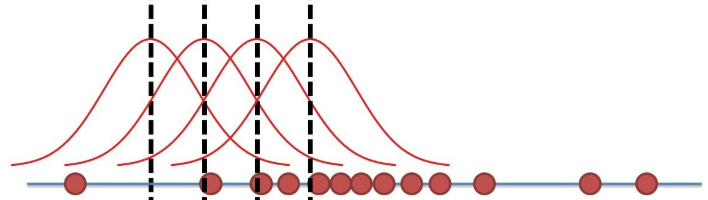
\includegraphics[width=1\linewidth]{MLE_pic1.png}
\end{figure}
\end{frame}
% ------------------------------------------------------------
\begin{frame}{A brief note on Maximum Likelihood Estimation (MLE)}

\textbf{Intuition:}
\begin{itemize}
    \item Pick parameters that make the model’s implied residuals “as close as possible” to white noise.
    \item Equivalent to minimizing the sum of squared innovations under normality.
    \item MLE automatically accounts for the correlation structure (unlike OLS).
\end{itemize}

\textbf{\textit{For AR models, conditional MLE $=$ OLS exactly under Gaussian errors. For MA/ARMA, conditional MLE $=$ NLS; both are asymptotically equivalent and efficient.}}
\end{frame}




% ------------------------------------------------------------
\section{Selection}

\begin{frame}{Model Selection}
\small

\textbf{Motivation: the bias-variance trade-off}
\begin{itemize}
    \item In ARMA modelling, we must choose the lag orders $(p,q)$.
    \item Higher $(p,q)$ always increases in-sample fit (the likelihood $\ell(\hat\theta)$ increases as the model becomes more flexible). But adding parameters also increases sampling uncertainty and may overfit random noise → higher variance of estimates, spurious dynamics, poor out-of-sample performance.
    \item Too few lags → underfit (bias), especially for new data; too many → overfit the noise (variance)\footnote{\footnotesize Adding parameters without increasing data \textbf{dilutes information per $\hat{\theta}$.}}
\end{itemize}
\textbf{Total error = bias + variance:}
\[
\text{MSE}(\hat{y}) 
= \underbrace{\text{Bias}^2}_{\text{underfit}} 
+ \underbrace{\text{Variance}}_{\text{overfit}} 
+ \sigma^2_\text{noise}.
\]
\textbf{Information criteria (based on maximized log-likelihood $\ell(\hat\theta)$):}
\[
\text{AIC} = -2\ell(\hat\theta) + 2k,
\qquad
\text{BIC} = -2\ell(\hat\theta) + k \log T,
\]
where $k$ = number of estimated parameters, $T$ = sample size.
\end{frame}

% ------------------------------------------------------------
\begin{frame}{Model Selection}
\small
\textbf{Interpretation:}
\begin{itemize}
    \item The first term ($-2\ell$) rewards fit (larger likelihood = better fit).
    \item The second term penalizes model complexity ($k$ parameters).
    \item AIC uses a lighter penalty → tends to favor richer models.  
    \item BIC penalizes complexity more strongly → favors simpler models.
    \item Select the model with the \textbf{lowest} criterion value.
\end{itemize}

\textbf{Other selection tools (for robustness):}
\begin{itemize}
    \item Hannan-Quinn criterion (HQC): intermediate penalty  
          $\text{HQC} = -2\ell(\hat\theta) + 2k \log\!\log T$.
\end{itemize}


\end{frame}

% ------------------------------------------------------------
\begin{frame}{Practical Model Selection Workflow}
\small

\textbf{Step 1 - Visual identification:}
\begin{itemize}
    \item Examine ACF / PACF of $X_t$ for first guesses of $(p,q)$.
    \item AR($p$): PACF cuts off at $p$, ACF decays.  
    \item   MA($q$): ACF cuts off at $q$, PACF decays.
\end{itemize}

\pause
\textbf{Step 2 - Statistical selection:}
\begin{enumerate}
    \item Estimate ARMA$(p,q)$ over a grid of plausible orders (e.g. 0-4).
    \item Compute AIC, BIC, HQC for each model.
    \item Choose $(p,q)$ minimizing the preferred criterion.
\end{enumerate}
\end{frame}


% ------------------------------------------------------------
\begin{frame}{Practical Model Selection Workflow}
\small

\textbf{Step 3 - Model validation:}
\begin{itemize}
    \item Check \textbf{residual} ACF → should collapse to 0 (i.e. residuals = white noise).
    \item \textbf{Ljung-Box (or other \textit{Portmanteau} test like old Box-Pierce)} test for residual autocorrelation (if white noise: no AC). \textbf{H0: $\rho_{\varepsilon}(h) = 0$ for $h = 1,\ldots,m$; H1: $\exists\, h \in\{1,\ldots,m\}$ s.t.\ $\rho_{\varepsilon}(h) \neq 0$} (choice of $m$: typically $\lfloor \ln T \rfloor$ or $\min(T/5, 40)$).
    \item Compare AIC/BIC with alternative diagnostics:
      \begin{itemize}
          \item Likelihood-ratio test for nested models (e.g. AR(1) $\subset$ AR(2)).
          \item Out-of-sample forecast errors (take the model which minimizes RMSE etc...)
          \item Rolling backtesting (= rolling cross-validation):
          \begin{itemize}
              \item Split sample: estimate on training set, test predictive accuracy on validation set, and do this with a rolling window (to avoid arbitrary separation $t$).
          \end{itemize}
      \end{itemize}
\end{itemize}

\textbf{Workflow summary:}
\[
\text{ACF/PACF (identify)} 
\;\Rightarrow\;
\text{AIC/BIC (select)} 
\;\Rightarrow\;
\text{Residual diagnostics (validate)}.
\]
\end{frame}

\begin{frame}{Practical Model Selection Workflow}
\small
\textbf{Step 4 - Normality check of residuals}
\begin{itemize}
    \item Even if residuals are uncorrelated, they may not be Gaussian.
\item This matters if you rely on MLE inference or confidence intervals (which assume normality).
\item Jarque-Bera normality test (or Shapiro if small sample, Kolmogorov for tail sensitivity). 
\item Q-Q Plot (Quantile-Quantile plot)
\begin{itemize}
    \item Compare empirical quantiles of residuals to theoretical normal quantiles.
\end{itemize}
\begin{itemize}
    \item Straight 45° line $\Longrightarrow$ normal residuals.
\end{itemize}
\begin{itemize}
    \item S-shaped $\Longrightarrow$ heavy tails or skewness
    \item Or plot residual histogram too (must be centered on 0 and look normal).
\end{itemize}
\end{itemize}
\end{frame}

\begin{frame}{Residuals Diagnostics 1 (Non-autocorrelation)}
\begin{figure}
    \centering
    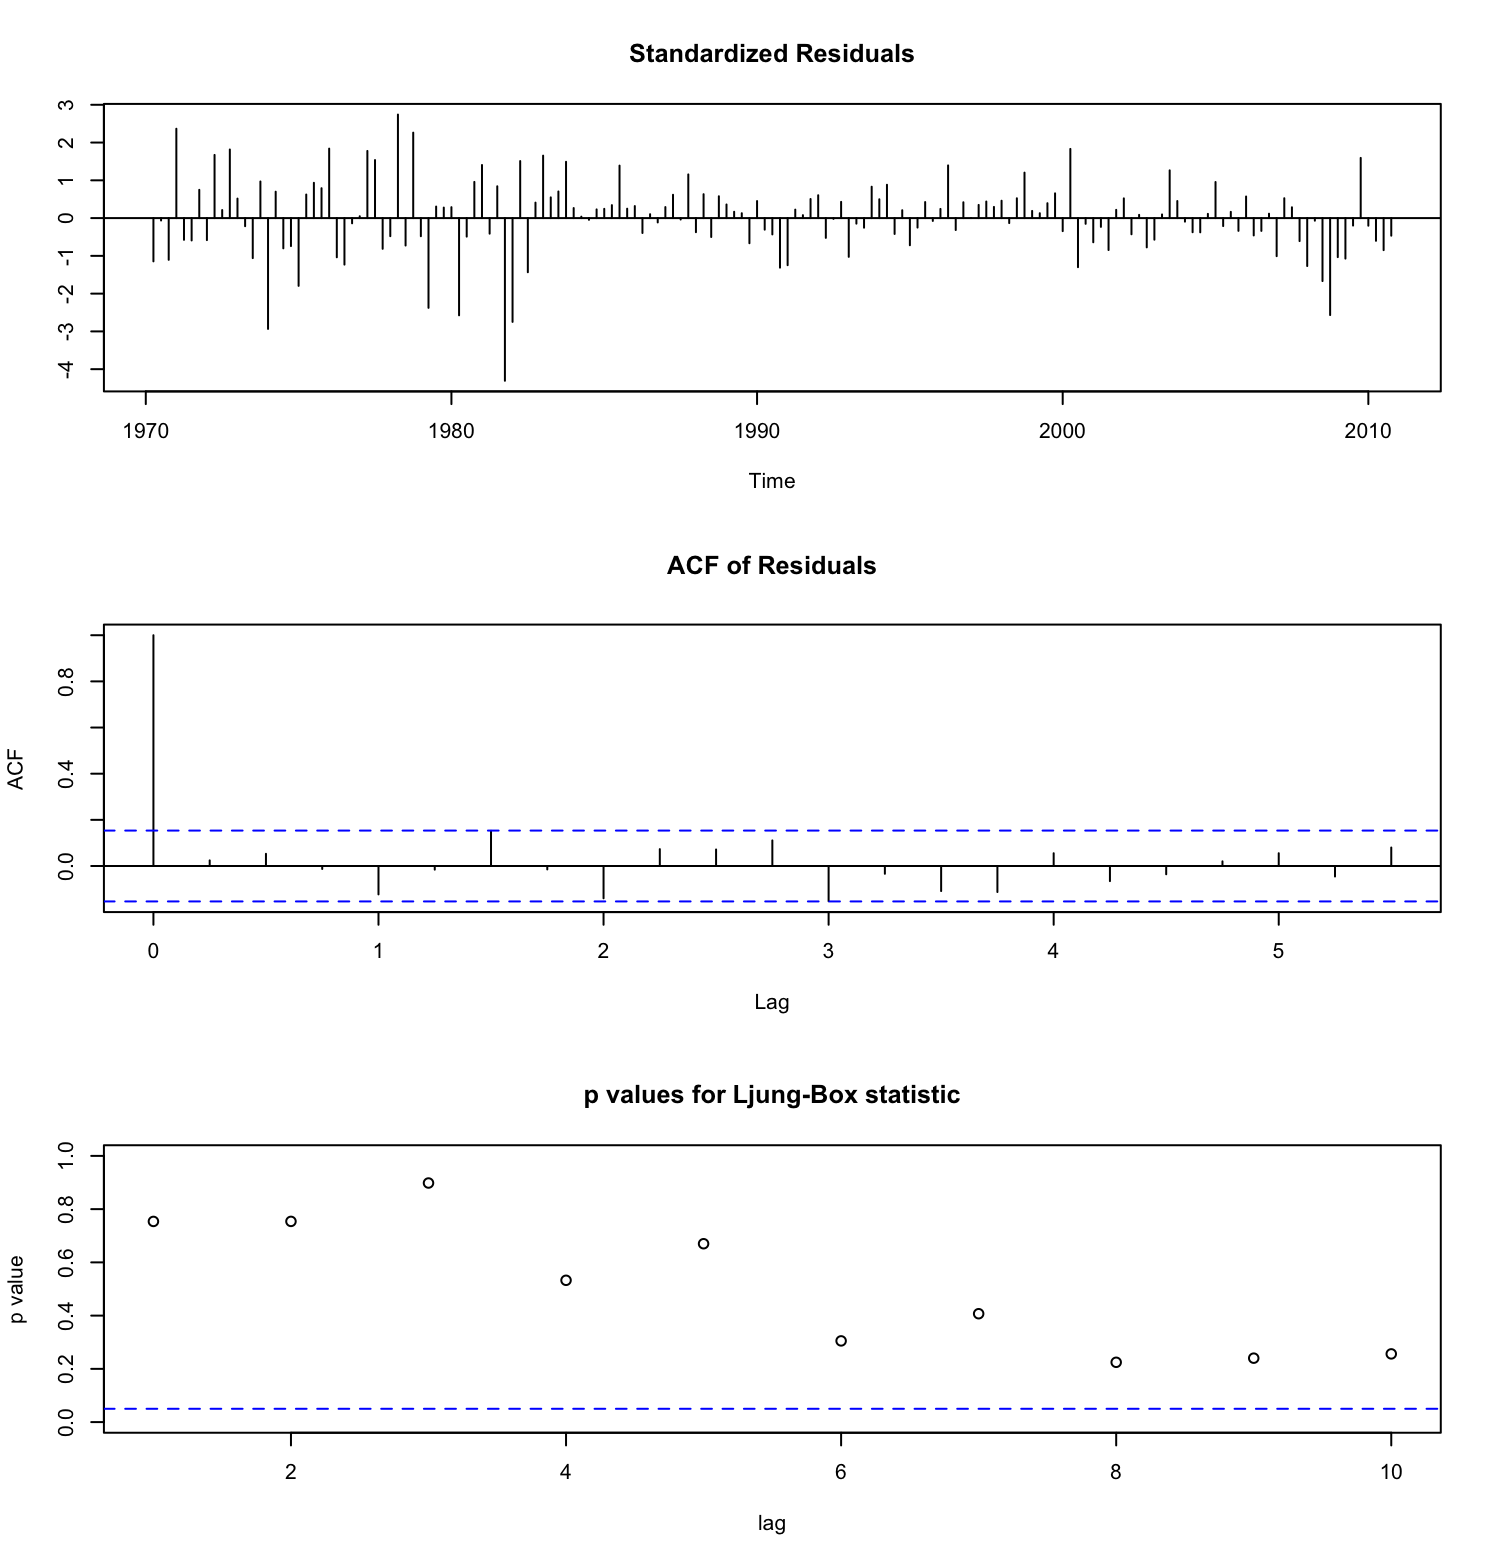
\includegraphics[width=0.7\linewidth]{residual ACF.png}
\end{figure}
    
\end{frame}

\begin{frame}{Residuals Diagnostics 2 (Normality)}
\begin{figure}
    \centering
    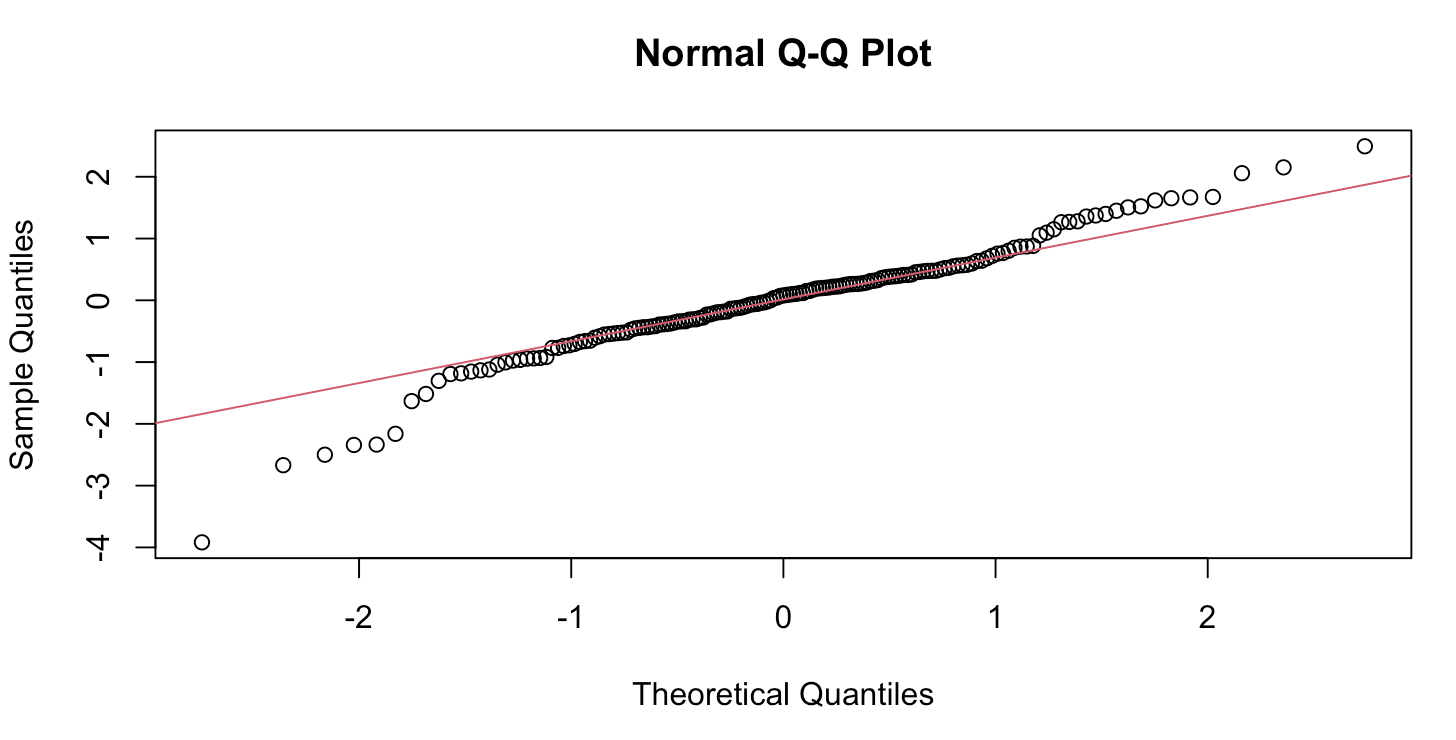
\includegraphics[width=1\linewidth]{normal_QQ.png}
\end{figure}
    
\end{frame}
% ------------------------------------------------------------


\begin{frame}{When AR? When MA? When ARMA?}
\small
\textbf{Must follow the Model Selection Worklow supra!} But:


\textbf{Autoregressive (AR)} models:
\begin{itemize}
  \item Dependence through feedback from past values.
  \item Useful when persistence is gradual and long-lived.
  \item ACF decays slowly, PACF cuts off $\rightarrow$ \emph{mean-reverting dynamics}.
\end{itemize}

\textbf{Moving-Average (MA)} models:
\begin{itemize}
  \item Dependence through past shocks.
  \item Capture short, transitory effects and noise smoothing.
  \item ACF cuts off sharply $\rightarrow$ \emph{finite memory}.
\end{itemize}

\textbf{ARMA models:}
\begin{itemize}
  \item Combine both persistence and short-term noise smoothing.
  \item Often needed because many real processes have both features:
        slow decay + finite-shock propagation.
  \item ARMA($p,q$) can approximate any stationary linear process efficiently
        (Box-Jenkins philosophy).
\end{itemize}
\end{frame}


\section{Forecasting}

\begin{frame}{Forecasting in AR Models (intuition)}
\small

\textbf{Key idea:} Future values depend on past values and future shocks.  
When forecasting, future shocks are unknown $\Rightarrow$ replace them by their expectation (0).

\textbf{Goal:} predict $X_{T+h}$ using available information $\mathcal{I}_T = \{X_1,\dots,X_T\}$.

\medskip
\textbf{Example: AR(1) $X_t = \phi X_{t-1} + \varepsilon_t$}

\underline{One-step ahead:} $\hat X_{T}(1) = \phi X_T$

\underline{Two-steps ahead:} $\hat X_{T}(2) = \phi \hat X_{T}(1) = \phi^2 X_T$. \textbf{Converges to... $0$ (or mean $m$ if any) with $h$}

General recursion:
\[
\hat X_{T}(h) = \phi^h X_T
\]

\medskip
\textbf{Example: AR(2)} $X_t = \phi_1 X_{t-1} + \phi_2 X_{t-2} + \varepsilon_t$

\underline{One-step ahead:} $\hat X_{T}(1) = \phi_1 X_T + \phi_2 X_{T-1}$ 

\underline{Two-steps ahead:} $\hat X_{T}(2) = \phi_1 \hat X_{T}(1) + \phi_2 X_T$

\underline{Three-steps: $\hat X_{T}(3) = \phi_1 \hat X_{T}(2) + \phi_2 \hat X_{T}(1)$}

\end{frame}

\begin{frame}{Forecasting in ARMA Models: General Case}
\small

\textbf{Optimal predictor (i.e. which has minimum MSE)} $\hat{X}_{T}(h) = \mathbb{E}[X_{T+h} \mid \mathcal{I}_T]$
\textbf{is ARMA($p,q$). One-step ahead forecast:}
\[
\hat{X}_{T}(1)
= \hat\mu
+ \sum_{i=1}^{p} \hat\phi_i X_{T-i+1}
+ \sum_{j=1}^{q} \hat\theta_j \hat\varepsilon_{T-j+1}
\]

\medskip
\textbf{For $h \ge 2$:} future shocks unknown $\Rightarrow$ set $\varepsilon_{T+k}=0$ for $k>0$.

\[
\hat X_T(h)
=
\underbrace{\hat\mu}_{\text{long-run mean}}
\;+\;
\underbrace{\sum_{i=1}^{p} \hat\phi_i \, \hat X_T(h-i)}_{\text{forecast using past, \textbf{then} previous forecasts}}
\;+\;
\underbrace{\sum_{j=1}^{\min(h-1,q)} \hat\theta_j \, \hat\varepsilon_{T+h-j}}_{\text{only use shocks that\textbf{ occurred}}}
\]


\medskip
\textbf{Forecast error:} $e_{T+h|T}
= X_{T+h} - \hat X_T(h)
= \sum_{i=0}^{h-1} \psi_i \varepsilon_{T+h-i}$

\[
\mathrm{Var}(e_{T+h|T})
= \sigma^2 \sum_{i=0}^{h-1} \psi_i^2
\]

\textbf{$\Rightarrow$ Forecast uncertainty (i.e. variance of forecast error) grows with $h$.}
\end{frame}


\begin{frame}{Forecasting in ARMA Models: Theoretical Framework}
\small

\textbf{$\Longrightarrow$ Variance of forecast error grows with horizon $h$.}

Remember, stationary thus the impact of a shock $\varepsilon$ is transitory:
    \[
        X_{t+h} = m + \sum_{k=0}^{\infty} \theta_k \varepsilon_{t+h-k}, 
        \quad \theta_h \to 0 \text{ as } h \to \infty.
    \]

So, what will be your forecast of $X_{t+h}$ as $h\to \infty$?
\end{frame}




\begin{frame}{Evaluating Forecast Accuracy}
\small
\textbf{Main criteria:}
\[
\text{ME} = \mathbb{E}[e_{T+h}], \quad
\text{MAE} = \mathbb{E}[|e_{T+h}|], \quad
\text{MSE} = \mathbb{E}[e_{T+h}^2], \quad
\text{RMSE} = \sqrt{\text{MSE}}.
\]
Empirical estimate:
\[
\widehat{\text{MSE}}(h) = \frac{1}{H}\sum_{k=1}^{H} (x_{T+k} - \hat{x}_{T+k})^2.
\]

\pause
\textbf{Interpretation:}
\begin{itemize}
    \item ME $\Rightarrow$ bias of forecasts (signs can cancel out errors).
    \item RMSE $\Rightarrow$ overall accuracy (quadratic loss, thus more sensitive to outliers).
    \item Compare models: lower RMSE $\Rightarrow$ better predictive performance.
\end{itemize}

\pause
\textbf{Cross-validation / backtesting:}
Use an expanding (or rolling) window to evaluate out-of-sample forecast errors.
\end{frame}


\begin{frame}{Forecast Uncertainty and Confidence Intervals}
\small
\textbf{Under Gaussian errors:}
\[
\hat{X}_T(h) \pm z_{1-\alpha/2}\,\hat{\sigma}_\varepsilon
\sqrt{\sum_{i=0}^{h-1} \hat{\psi}_i^2}
\]
\begin{itemize}
  \item Wider intervals as $h$ increases (forecast uncertainty accumulates).

\end{itemize}

\pause
\textbf{When distribution unknown: Bootstrap approach}
\begin{enumerate}
  \item Resample residuals $\hat{\varepsilon}_t^*$ with replacement to obtain their empirical distribution (Gaussian assumption: often incorrect!)
  \item Generate pseudo-series and re-estimate parameters.
  \item Compute empirical distribution of $\hat{X}_T^*(h)$.
  \item Use percentiles to construct confidence intervals.
\end{enumerate}
\end{frame}


\begin{frame}{Monte Carlo vs.\ Bootstrap}
\small
\textbf{Monte Carlo simulation}
\begin{itemize}
  \item Assumes a known \textbf{data-generating process (DGP)}.
  \item Simulate many samples directly from this model.
  \item \emph{Example:} $X \sim N(0,1)$, draw samples of size $n$, compute $\bar X$.
\end{itemize}

\pause
\textbf{Bootstrap}
\begin{itemize}
  \item Used when the true DGP is \textbf{unknown}, to check robustness to sampling variability.
  \item \textbf{Idea (Efron, 1979):} Use the data as a proxy for the population.  
  \item \textit{"If we cannot resample the population, we resample the sample." }
  \item Resample \emph{with replacement} from the data, recompute statistic. 
  \item \emph{Example:} wages of 400 workers; resample to approximate sampling distribution of the median and build percentile CIs. Same for time series uncertainty bands in forecasting.
\end{itemize}

\pause
\begin{itemize}
  \item All bootstraps are Monte Carlo resampling schemes.
  \item But not all Monte Carlo simulations are bootstraps.
\end{itemize}
\end{frame}


\section{Conclusion}

\begin{frame}{From ARMA to ARIMA Models}
\small
Many macroeconomic and financial time series are \textbf{non-stationary} (contain unit roots).

\pause
\textbf{Idea:} difference the series until stationarity, then model with ARMA.
\[
(1 - L)^d X_t = \text{stationary process}, \qquad
\Rightarrow X_t \sim \text{ARIMA}(p,d,q).
\]
$d$ is the order of integration (e.g. if $d=2$, you need to take the first difference of the first difference to obtain a stationary process). 

\textbf{Example:}
\begin{itemize}
    \item If $X_t$ is a random walk: $(1 - L)X_t = \varepsilon_t$ → $d=1$, ARIMA(0,1,0).
    \item If $(1-L)X_t$ follows ARMA(1,1) → ARIMA(1,1,1). If log: growth rate.
    \item If $(1-L)^2X_t$ (i.e. $\Delta^2 X_t = (X_t - X_{t-1}) - (X_{t-1} - X_{t-2})$) is stationary, thus $d=2$. If log: acceleration rate (growth rate of the growth rate).
\end{itemize}

\textbf{Interpretation:}
Differencing removes trends $\Longrightarrow$ ARIMA generalizes ARMA to non-stationary data.

Example of a $I(2)$ series: Price level $\Rightarrow$ Inflation $\Rightarrow$ Change rate of Inflation
\end{frame}


\begin{frame}{Summary of the Workflow (Box-Jenkins Approach)}
\footnotesize
\begin{enumerate}
  \item \textbf{Visual Inspection \& Stationarity Check}
    \begin{itemize}
      \item Plot the series and ACF, visually inspect mean/variance constancy and ACF decay (or breaks, trends...).
      \item Run \textbf{unit root tests} (ADF, PP, DF-GLS, KPSS). If non-statio $\to$ difference ($\Delta X_t$) / remove deterministic trend, check unit roots.
    \end{itemize}

  \item \textbf{Identify Model Orders $(p,q)$}
    \begin{itemize}
      \item Use \textbf{ACF/PACF} patterns:
        AR($p$) $\to$ PACF cutoff; MA($q$) $\to$ ACF cutoff; ARMA $\to$ both decay.
      \item Confirm visually that stationarity now holds.
    \end{itemize}

  \item \textbf{Estimate Parameters}
    \begin{itemize}
      \item AR($p$): OLS (consistent under stationarity).
      \item MA/ARMA: Maximum Likelihood or Nonlinear Least Squares.
    \end{itemize}

  \item \textbf{Model Selection \& Validation}
    \begin{itemize}
      \item Compare models via AIC, BIC, HQC (bias-variance trade-off).
      \item Check residuals $\varepsilon_t$: white noise? (Ljung-Box, ACF of residuals)
      \item Check normality (Jarque-Bera, Q-Q plot).
    \end{itemize}

  \item \textbf{Forecasting \& Evaluation:} Compute forecasts $\hat X_{T}(h)$ and forecast intervals. And evaluate predictive accuracy (RMSE, MAPE) with rolling windows.
\end{enumerate}
\end{frame}



\begin{frame}{Summary of the Workflow (Box-Jenkins Approach)}

\textbf{NB:} if integrated at order one ($I(1)$) i.e. if you have taken the growth rate for ARIMA estimation and forecast, you can come back to levels by cumulating the growth rates!
\medskip
And if you have just remove the deterministic trend, you can just add it again (and its continuation if forecast).

\medskip

\textbf{Next two sessions: }
\begin{enumerate}
    \item How to consider a \textbf{multivariate} framework? (i.e. \textit{\textbf{vector} auto-regression - VAR})
    \item Can we not only forecast the future, but also \textbf{simulate the impact of a policy / a shock} in causal, "structural" way? (i.e. \textit{impulse response function - IRF - in Structural VAR})
    \item Can we quantify the \textbf{contribution of each variable} to the overall variance? (i.e. \textit{variance decomposition})
\end{enumerate}
\end{frame}


\end{document}

